\section{Dataset Analysis}
The subsequent analysis in the report employs the RNA-Seq dataset of the human dorsal striatum, which is comprised of 18 cohorts of individuals diagnosed with Bipolar Disorder (BD) and 18 control subjects.
\subsection{Origin and Context of DataSet}
As stated by R. Pacifico and RL Davis in \cite{pacifico2017transcriptome}, the data is derived from 36 frozen postmortem human striatum samples provided by the Harvard Brain Tissue Resource Center. These samples are accompanied by information regarding the age, sex, and postmortem interval (PMI) of sample collection from the donors. The original study excluded one outlier control sample, designated as C 28, and conducted differential gene expression (DGE) analysis on 35 samples (18 bipolar and 17 control). The covariates (age, sex, PMI, and RIN) for both the bipolar and control groups were not significantly different from each other. This report presents two results: one considering the inclusion of the C 28 control sample and another considering its exclusion. The objective is to observe the differences in the outcome of the DGE analysis. In bipolar disorder, it is especially important to consider how long the manic episode continues, and the data has been normalized to account for this constraint.
\begin{table}[H]
\centering
\begin{tabular}{llrlrr}
\toprule
geo accession & title & age (years) & Sex & postmortem interval (hours) & rin \\
\midrule
GSM2124738 & control-2 & 83 & male & 13.000000 & 3.700000 \\
GSM2124739 & control-3 & 55 & female & 21.660000 & 2.900000 \\
GSM2124771 & bipolar-34 & 80 & female & 13.660000 & 3.600000 \\
GSM2124772 & bipolar-37 & 61 & female & 16.630000 & 2.200000 \\
GSM2124773 & bipolar-40 & 77 & female & 29.580000 & 6.700000 \\
\bottomrule
\end{tabular}
\caption{Part of sampled cohort data}
\label{tab:metadata_entr}
\end{table}
Table \ref{tab:metadata_entr} refers to a part of the cohort data, which provides a more concrete description of the dataset.
\begin{table}[H]
\centering
\begin{tabular}{ccccc}
\toprule
Group & Age ($\mu \pm \sigma$) & Sex (Male, Female) & PMI ($\mu \pm \sigma$) & RIN ($\mu \pm \sigma$) \\
\midrule
Control & 65 $\pm$ 15.7 & 7, 11 & 22.8 $\pm$ 6.4 & 4 $\pm$ 1.7 \\
Cohort & 69.7 $\pm$ 15.3 & 6, 12 & 25.1 $\pm$ 15.8 & 3.9 $\pm$ 1.5 \\
\bottomrule
\end{tabular}
\caption{Summary of cohorts}
\label{table:cohort_info}
\end{table}
\noindent Table \ref{table:cohort_info} presents a summary of the most notable statistics from the dataset pertaining to each cohort and control group. It should be noted that these statistics exclude the effect of an outlier, C\_28, from the sample.

\subsection{Data Preprocessing}
This section discusses the specific data pre-processing operations that are outlined in the earlier section while introducing the workflow. Let us start by the Illumina high-throughput sequencing data.

\subsubsection{Illumina RNA Sequencing Data}
RNA-Seq data, or RNA sequencing data, is the collection of information generated by sequencing the RNA molecules within a biological sample. This data provides insights into gene expression, revealing which genes are active, to what extent, and under what conditions. RNA-Seq data can be obtained through several methods, including single-end and paired-end sequencing. The process involves extracting RNA from the sample, converting it into complementary DNA (cDNA) using reverse transcription, and then sequencing the cDNA using high-throughput sequencing technologies. The figure \ref{fig:hiseq_machine} illustrates the procedure of obtaining RNA-Seq data from an RNA sample using the Illumina HiSeq-2000, which is one of the most commonly used sequencing machines. The high-throughput sequencing FASTQ dataset used for the analysis is also sequenced by Illumina HiSeq-2000.
\begin{figure}[H]
    \centering
    \subfloat[\centering Sequencing the RNA sample on Illumina HiSeq-2000]{{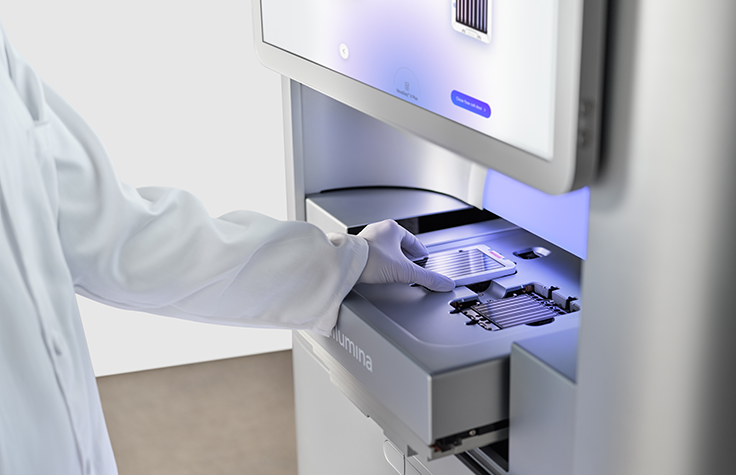
\includegraphics[width=7cm]{workflow_img/seq-illumina-technology.png} }}%
    \qquad
    \subfloat[\centering Illumina HiSeq-2000 Sequencing Machine]{{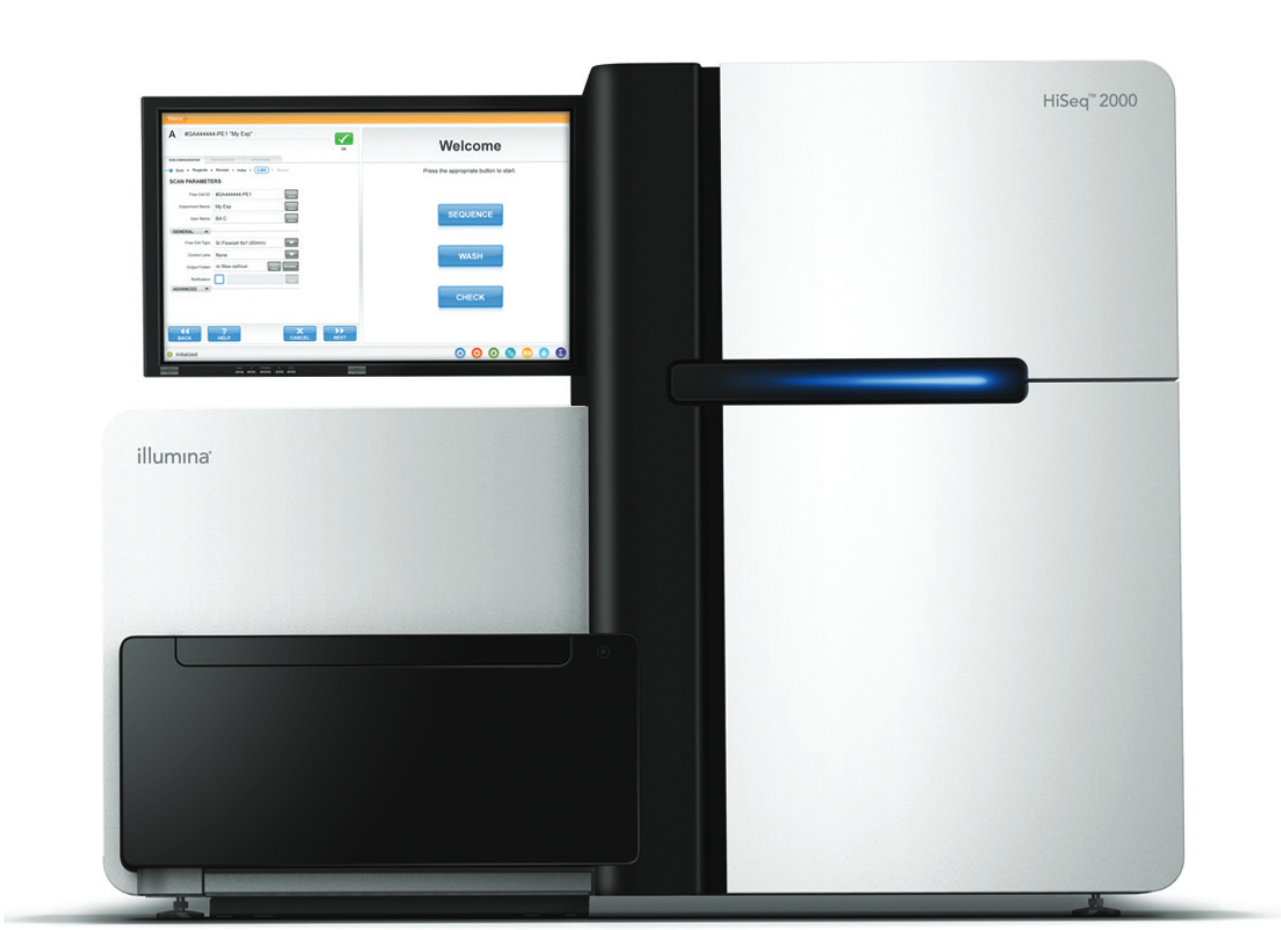
\includegraphics[width=7cm]{workflow_img/illumina-hiseq-3000.png}}}%
    \caption{High-throughput sequencing machine}
    \label{fig:hiseq_machine}
\end{figure}
In most cases, the raw RNA-Seq data is available in the FASTQ format. The following code section \ref{code:sample-fastq} describes the typical FASTQ file of RNA-Seq data.
\begin{code}
\captionof{listing}{Sample FASTQ output}
\label{code:sample-fastq}
\begin{minted}{ada}
@SRR3393492.1 HISEQ:313:D2H4NACXX:2:1101:1200:1867 length=88
NTCCGTCTTGCGCCGGGCCAAGAATTTCACCTCTAGCGGCGCAATACGAATGCCCCCGGCCGGCCCTCTTAATCATGGCCTCAGTTCC
+SRR3393492.1 HISEQ:313:D2H4NACXX:2:1101:1200:1867 length=88
#11?7?;AAACCACAA)??ABA3>AAAB0=ABBB<A><AA################################################
\end{minted}
\end{code}
Each record in a FASTQ file consists of four lines, which are repeated for every sequence in the file. The above data represents a single record. The first line begins with @ and serves as the sequence identifier, providing a unique name for the read (\texttt{SRR3393492.1}) and additional metadata such as sequencing instrument (\texttt{HISEQ:313:D2H4NACXX}) and read length (\texttt{length=88}). The second line contains the raw nucleotide sequence (\texttt{NTCCGTCTTGCGCCGGGCCAAGAATT...}), representing the biological data obtained from the sequencing process. The third line starts with a + symbol and may either repeat the sequence identifier or remain blank, serving as a separator for the quality scores. The fourth line encodes the quality scores using ASCII characters (\texttt{\#11?7?;AAACCACAA)...}), which represent Phred scores for each nucleotide.

The Phred score is a numerical value used to represent the quality of a nucleotide base call. It is a logarithmic measure of the probability \(P\) that a base call is incorrect. Higher Phred scores indicate higher confidence in the accuracy of the base call. Given that \(P\) is the probability of the base call being incorrect, its Phred score \(Q = -10 \log_{10}(P)\) is computed and encoded into an ASCII character by adding \(33\) to it. For instance, the character \(I\), which corresponds to ASCII 73, indicates a Phred score of 40.

Our computational pipeline downloads all FASTQ files from the NCBI SRA database. These raw sequencing data is then assembled into SAM files via HISAT2.

\subsubsection{Sequence Alignment Data}  
Before performing the sequence alignment, it is essential to construct the reference genome database, which serves as the foundation for aligning sequencing reads. The computational pipeline generates the reference genome database from the NCBI *Homo sapiens* reference genome dataset using the following command:

\begin{minted}{shell}
    hisat2-build -p 32 "data/GCF_000001405.40_GRCh38.p14_genomic.fna" "ref_genome/ref_gen"
\end{minted}

In this command, \texttt{hisat2-build} creates index files necessary for alignment using 32 parallel threads (\texttt{-p 32}). The input file is the reference genome in \texttt{.fna} format, while the output consists of indexed files stored under the specified prefix \texttt{ref\_genome/ref\_gen}. These index files allow efficient alignment of sequencing reads to the reference genome.

Once the reference genome database has been constructed, the pipeline proceeds with the alignment of sequencing reads (in \texttt{FASTQ} format) against the reference genome using HISAT2. The following command is executed:

\begin{minted}{shell}
hisat2 -p 32 -x ref_genome/ref_gen -U "fastq_files/SRR3393492.fastq" \
       -S "alignment/SRR3393492.sam"
\end{minted}
In this alignment step, \texttt{-p 32} specifies the use of 32 threads for multi-threaded processing. The tag \texttt{-x} points to the prefix of the reference genome index files created in the previous step. Also, \texttt{-U} specifies the input file containing single-end sequencing reads (\texttt{SRR3393492.fastq}). Finally, \texttt{-S} indicates the output file path, where the alignment results are stored in SAM (Sequence Alignment/Map) format.

The resulting SAM file contains essential information for each aligned read, including its position on the reference genome, alignment flags, mapping quality scores, and more. The header section of the SAM file provides metadata about the reference genome sequences used during alignment. Table~\ref{table:sam_header} shows the first few rows of the header section from the processed SAM file corresponding to cohort ID \texttt{SRR3393492}.
\begin{table}[H]
    \centering
    \begin{tabular}{cll}
        \toprule
        Record Type & Sequence Name (SN) & Sequence Length (LN) \\
        \midrule
        @SQ & NC\_000001.11 & 248956422 \\
        @SQ & NT\_187361.1 & 175055 \\
        @SQ & NT\_187362.1 & 32032 \\
        @SQ & NT\_187363.1 & 127682 \\
        @SQ & NT\_187364.1 & 66860 \\
        @SQ & NT\_187365.1 & 40176 \\
        \bottomrule
    \end{tabular}
    \caption{Header section of the SAM file for \texttt{SRR3393492}.}
    \label{table:sam_header}
\end{table}
This SAM file header section begins with lines prefixed by the @ symbol, which provide information about the reference genome sequences used for alignment. Each line in the header contains the following fields.

First, the record type field is specified by the tag \texttt{@SQ} which indicates a sequence record that describes a sequence from the reference genome. Next, sequence name (SN) field provides the name or unique identifier of the reference genome sequence. For instance, \texttt{NC\_000001.11} corresponds to the primary assembly of chromosome 1. Other identifiers, such as \texttt{NT\_187361.1}, represent unplaced or alternate contigs. Lastly, sequence length (LM) field specifies the length of the corresponding sequence in base pairs (bp). For example, chromosome 1 (\texttt{NC\_000001.11}) has a length of 248,956,422 bp. This header ensures proper mapping of sequencing reads to their corresponding positions in the reference genome, while also enabling downstream tools to interpret the aligned data accurately.



\subsubsection{Raw Read Count Data}
For each alignment SAM file, the pipeline performs read count generation by executing the following command.
\begin{minted}{shell}
htseq-count "alignment/SRR3393492.sam" "data/GCF_000001405.40_GRCh38.p14_genomic.gtf.gz"
            -f sam -r pos -i gene_id -t exon -n 32 > "transcripts/SRR3393492.csv"
\end{minted}
\subsubsection{Raw Read Count Data}  
For each alignment SAM file, the pipeline generates raw read count data using the \texttt{htseq-count} tool. This process quantifies the number of reads aligned to annotated genomic features such as exons, enabling downstream analyses like differential gene expression. The pipeline executes the following command.
\begin{minted}{shell}
htseq-count "alignment/SRR3393492.sam" "data/GCF_000001405.40_GRCh38.p14_genomic.gtf.gz" \
            -f sam -r pos -i gene_id -t exon -n 32 > "transcripts/SRR3393492.csv"
\end{minted}
Let us take a closer look at each argument in the above command. First, \texttt{"alignment/SRR3393492.sam"} specifies the input SAM file containing aligned sequencing reads. Notice that each read in this file has already been mapped to the reference genome using HISAT2. Next, \texttt{"data/GCF\_000001405.40\_GRCh38.p14\_genomic.gtf.gz"} refers to the gene annotation file in \texttt{GTF} (Gene Transfer Format). This file contains information about genomic features, such as gene locations, transcript structures, and exons, which are essential for counting reads overlapping these regions.

HTSeq can process different alignment formats such as SAM and BAM. The argument \texttt{-f sam} specifies in detail that the input file format is SAM. Next, \texttt{-r pos} option instructs HTSeq to process reads in positional order, sorted by genomic position, for efficiency during the counting procedure. This ensures optimal handling of the aligned data.

Next, \texttt{-i gene\_id} option identifies the attribute in the GTF file to be used as the feature ID. In this case, \texttt{gene\_id} is used to group reads by gene identifiers. Following argument \texttt{-t exon} specifies that the counting should occur at the \texttt{exon} feature level. By enabling this option, reads overlapping exonic regions will be aggregated to calculate gene-level counts. Similar to HISAT2, HTSeq-count also support multi-threading, and \texttt{-n 32} enables multi-threading with 32 threads to accelerate the counting process. Then, the last argument \texttt{> "transcripts/SRR3393492.csv"} simply redirects the output to a CSV file. Each line of this file contains the feature ID (gene ID) and its corresponding raw read count.

In more detail, HTSeq-count library generates read counts in the following process. First, \texttt{htseq-count} parses the GTF file to extract genomic feature coordinates such as exons and their associated identifiers like \texttt{gene\_id}. Here, each genomic feature is treated as a region of interest for counting reads. This step is called \emph{Feature Extraction}. Then, for each read in the SAM file, \texttt{htseq-count} determines whether the read overlaps any genomic feature based on its aligned position. Overlap is determined using the genomic coordinates of the read and features.

Next step is referred to \emph{Feature Assignment}. If a read overlaps exactly one feature (e.g., an exon), it is assigned to that feature. Reads overlapping multiple features are handled based on the default “union” mode, where reads are only counted if they unambiguously belong to a single feature. 

Once the assignment is complete, Reads assigned to individual exons are aggregated at the gene level using the \texttt{gene\_id} attribute to calculate raw gene-level counts. Afterwards, HTSeq-count creates the final output is a tab-delimited file where each line contains a gene ID and its corresponding raw read count.

Then, the raw expression data, that is, the dataset of raw read counts per gene, is obtained by merging all read counts CSV files obtained from the \texttt{HTSeq-count} library. Note that this data can also be retrieved from the supplementary files section of the Gene Expression Omnibus (GEO) repository. The relevant data can be accessed via the following URL: \url{https://www.ncbi.nlm.nih.gov/geo/query/acc.cgi?acc=GSE80336}. The respective RNA-Seq data for over 36 samples have been sequenced using the Illumina HiSeq 2000 platform. Table \ref{table:countdata_info} provides a subset of the raw count information.
\begin{table}[H]
\centering
\begin{tabular}{clcccrrrr}
\toprule
Ensembl\_ID & GeneSymbol & Biotype & Chromosome & C\_2 & C\_3 & BD\_34 & BD\_37 & BD\_40 \\
\midrule
ENSG00000000003 & TSPAN6 & protein\_coding & X & 87 & 68 & 128 & 91 & 99 \\
ENSG00000000005 & TNMD & protein\_coding & X & 0 & 0 & 0 & 2 & 1 \\
ENSG00000000419 & DPM1 & protein\_coding & 20 & 129 & 195 & 197 & 149 & 124 \\
\vdots & \vdots & \vdots & \vdots & \vdots & \vdots & \vdots & \vdots & \vdots \\
ENSG00000001167 & NFYA & protein\_coding & 6 & 363 & 455 & 594 & 464 & 413 \\
\bottomrule
\end{tabular}
\caption{Raw count data}
\label{table:countdata_info}
\end{table}
In this dataset, the Ensembl ID serves as the unique, stable identifier assigned to each gene, transcript, protein, and exon. Additionally, the letters "C" and "BD," utilized in column labels, represent abbreviations for "control" and "bipolar disorder," respectively. As this dataset is derived from \emph{homo sapiens} samples, chromosome attributes indicate the chromosome to which the selected gene belongs, including autosomes 1-22 or sex chromosomes X or Y.